\section{Motivation}
While the output from Grad-CAM does not provide a good insight into what the segmentation neural network is doing, the RISE output is quite usable. When evaluation an interpretability method, not only the method itself but also the trained neural network is analyzed. It is therefore possible that a good method returns bad results because the neural network is of low quality. We therefore decided to generate an artificial dataset (a "toy" example) where there is no doubt about its quality.


\section{Introduction}
\nblink{brats/08\_testnet\_generate.ipynb}
\nblink{brats/09\_testnet\_train.ipynb}


\begin{figure}[H]
    \centering
    \begin{subfigure}{.5\textwidth}
        \centering
        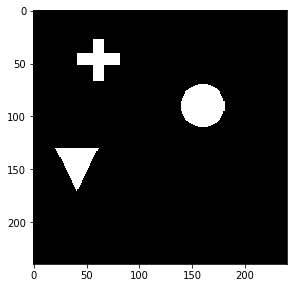
\includegraphics[width=5cm]{chapters/05_testnet/images/testnet_a-0.png}
        \caption{Input image}
    \end{subfigure}%
    \begin{subfigure}{.5\textwidth}
        \centering
        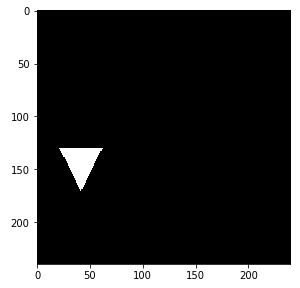
\includegraphics[width=5cm]{chapters/05_testnet/images/testnet_a-1.png}
        \caption{Output segment}
    \end{subfigure}
    \caption{Testnet with circle: The input image contains a circle on the right, therefore the triangle should be segmented}
\end{figure}

\begin{figure}[H]
    \centering
    \begin{subfigure}{.5\textwidth}
        \centering
        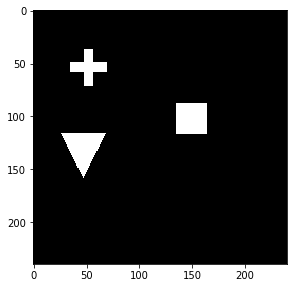
\includegraphics[width=5cm]{chapters/05_testnet/images/testnet_b-0.png}
        \caption{Input image}
    \end{subfigure}%
    \begin{subfigure}{.5\textwidth}
        \centering
        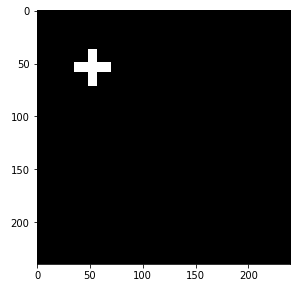
\includegraphics[width=5cm]{chapters/05_testnet/images/testnet_b-1.png}
        \caption{Output segment}
    \end{subfigure}
    \caption{Testnet with cube: The input image contains a square on the right, therefore the cross should be segmented}
\end{figure}


\subsection{Results}

\section{Applying RISE}
\nblink{brats/brats/10\_testnet\_rise.ipynb}
\nblink{brats/brats/11\_testnet\_rise\_segment\_ignore.ipynb}


\subsection{Results}
TODO Multipixel RISE results

\subsection{Discussion}
TODO: something is visible, but not good enough
